
\section{Introduction}
\label{sec:introduction}

Many software applications support
configuration options that allow users to
customize their behavior. This flexibility has a cost: when something
goes wrong, diagnosing a configuration error can be both time-consuming
and frustrating. Technical support contributes 17\% of the total cost of ownership of
today's software, and troubleshooting misconfigurations
is a large part of technical support~\cite{confevidence}.

Software misconfigurations may lead to incorrect output (i.e., non-crashing
errors) or to unexpected termination
(i.e., crashing errors).  Even when an application outputs an error
message, it is often cryptic or misleading~\cite{Yin:2011:ESC, Attariyan:2010:ACT, Hubaux:2012, rangefix}.
Users may not even think of configuration as a cause of their problem.
% Thus, users must search manuals, FAQs, and online forums to find potential
% solutions.% to the problem. %$\blacksquare$ this process is frustrating..
\looseness=-1

\subsection{Motivating Example}
\label{sec:mot}

%This section describes a real scenario in which we used \ourtool to solve %a configuration problem. 
We next describe a real scenario in which we used \ourtool to solve a configuration problem. 
We received a ``bug report'' against the Randoop
automated test generation tool~\cite{PachecoLET2007},
from a testing expert who had been using Randoop for quite a while.
The ``bug report'' indicated that Randoop terminated normally but
failed to generate tests for the NanoXML~\cite{nanoxml} program. 
%The symptom is that
%Randoop terminates normally but does not generate any tests.
%on NanoXML, it 

Although the reported problem is deterministic and fully-reproducible,
it is a silent, non-crashing failure and is
challenging to diagnose. Differing from
a crashing error, Randoop did not exhibit a crashing point, dump
 a stack trace, output an error message, or indicate suspicious program
variables that may have incorrect values. Lacking such information
makes many
techniques such as dynamic slicing~\cite{Zhang:2003:PDS},
dynamic information flow tracking~\cite{Attariyan:2010:ACT}, and
failure trace analysis~\cite{Rabkin:2011:PPC} inapplicable.
In addition, for this scenario, the person who reported the bug had already
minimized the bug report:  if any part of the 
configuration or input is removed, Randoop either crashes or
no longer exhibits this error.
This further makes 
search-based fault isolation techniques such as Delta debugging~\cite{Zeller:2002:ICC}
ineffective.
\looseness=-1

%there is no obvious testing oracle\todo{Why
%  not?  Wouldn't ``some output vs.\ no output'' be a testing oracle?} to check whether
%Randoop behaves as desired, which  Moreover, 

In fact, this bug report does not reveal a real bug
in the Randoop code. Its root cause is simply because
the user forgot to set one configuration option.
Despite the simplicity of the solution, to the best of our knowledge, no
existing configuration error diagnosis technique~\cite{Attariyan:2008:UCD, 
Whitaker:2004:CDS, Wang:2004:AMT,
Attariyan:2010:ACT, Rabkin:2011:PPC} can be directly applied.


%We reproduce this problem in a \ourtool-enabled environment.
%It determines which predicates exemplify the buggy behaviors.


\begin{figure}[t]
\begin{CodeOut}
\begin{alltt} 
Suspicious configuration option: maxsize

It affects the behavior of predicate:
"newSequence.size() > GenInputsAbstract.maxsize"
(line 312, class: randoop.ForwardGenerator) 

This predicate evaluates to true:
  3.3\% of the time in normal runs (3830 observations)
  32.5\% of the time in the undesired run (2898 observations)
\end{alltt}
\end{CodeOut}
\vspace*{-13pt}
\Caption{{\label{fig:output}
The top-ranked configuration option in \ourtool's error report
for the motivating example in Section~\ref{sec:mot}. The whole error
report contains 31 options. 
}} %\vspace{-5mm}
\end{figure}
%, this predicate evaluates to true:   (1315 observation%run, it evaluates to true:  (2727 observations)s)

As an alternative, we can use our technique (and its tool implementation \ourtool)
to diagnose and correct this problem. We first reproduced the
error in a \ourtool-instrumented Randoop version, then used \ourtool
to diagnose the error's root cause by analyzing the recorded execution profile.
\ourtool produced
a report (Figure~\ref{fig:output}) in the form of an ordered list of
suspicious configuration options that should be inspected.
The error report in Figure~\ref{fig:output} suggests that
a configuration option named
\CodeIn{maxsize} is the most likely one.
The report also provides relevant 
information to explain why: % about the reason why \CodeIn{maxsize} should be account for:
a program predicate affected by \CodeIn{maxsize} behaves dramatically
differently between the recorded undesired execution
and the correct executions found in \ourtool's database.
\looseness=-1

Figure~\ref{fig:example} shows the relevant code snippet
in Randoop.  When Randoop generates a new test (line 100, in the form of
a method-call sequence),
Randoop first compares its length with \CodeIn{maxsize}
(default value: 100). If the
generated sequence's length exceeds this pre-defined limit,
Randoop discards it to avoid length explosion in further
test generation.
Although \CodeIn{maxsize}'s default value was carefully chosen
by the Randoop developers
and works well for many programs (including those used to test
Randoop during its development), the generated sequences for NanoXML
are much longer than usual and using \CodeIn{maxsize}'s default value
results in 32.5\% of the generated sequences being discarded
(including sequences that the user wishes to remain).
\ourtool captures such abnormal behavior from Randoop's
silent failure, pinpoints the
\CodeIn{maxsize} option, and suggests the users to change its value.
The problem is resolved if
the user changes \CodeIn{maxsize} to a larger value, for example 1000.
\looseness=-1


%Guided by the report, we can further find out
%the root cause of Randoop's silent failure
%is because 

%and only 14.4\% of the generated sequences have been discarded.
%However,

%are discarded because the generated sequences are much longer.  

\begin{figure}[t]
\vspace{-2mm}
\small{In class: randoop.main.GenInputsAbstract}\\
%\small{//a configuration option to control a sequence's max length}
\vspace{-5mm}
\begin{CodeOut}
\begin{alltt}
     //{The maxsize configuration option. Default value: 100.}
157. public static int maxsize = readFromCommandLine(); 
\end{alltt}
\end{CodeOut}

{\small{In class: randoop.ForwardGenerator}}\\
\vspace{-5mm}
\begin{CodeOut}
\begin{alltt}
99.  public ExecutableSequence step() \ttlcb
100.   ExecutableSequence eSeq = createNewUniqueSequence();
101.   AbstractGenerator.currSeq = eSeq.sequence;
102.   eSeq.execute(executionVisitor);
103.   processSequence(eSeq);
104.   if (eSeq.sequence.hasActiveFlags()) \ttlcb
105.     componentManager.addGeneratedSequence(eSeq.sequence);
106.   \ttrcb
107.   return eSeq;
108. \ttrcb

310. private ExecutableSequence createNewUniqueSequence() \ttlcb
311.   Sequence newSequence = ...; //create a sequence
312.   if (newSequence.size() > GenInputsAbstract.maxsize) \ttlcb
313.     return null;
314.   \ttrcb
315.   if (this.allSequences.contains(newSequence)) \ttlcb
316.     return null;
317.   \ttrcb
318.   return new ExecutableSequence(newSequence);
319. \ttrcb
\end{alltt}
\end{CodeOut}
\tinystep
\vspace*{-3.0ex} \Caption{{\label{fig:example} 
Simplified code excerpt from Randoop~\cite{PachecoLET2007}
corresponding to the configuration problem reported in Figure~\ref{fig:output}.
%\todo{Need line number for \<int maxsize = ...> line at top.}
%A forward slice computed by the traditional slicing algorithm~\cite{Horwitz:1988:ISU}
%from the seed statement includes statements 2, 3,
%4, 5, 6, 7, 9, 13, 14, 16, 17, and 19.
%By contrast, a thin slice~\cite{Sridharan:2007}
%only contains line 13.
}} %\vspace{-1.8mm}
\end{figure}




%\vspace{1mm}
%\noindent \textbf{\textit{Our technique.}} 

\subsection{Diagnosing Configuration Errors}

Diagnosing a configuration error can be divided into two
separate tasks: identifying which specific configuration option is
responsible for the unexpected behavior, and determining a better value for
the configuration option. This paper addresses the former task: finding
the root cause of a configuration error.
%, and leave the later task
%of fixing


%The goal of \textbf{our technique} is to help users find solutions to the configuration
%problems they are facing.  
\textbf{Our technique} is designed to be used by system administrators
and end-users when they encounter an error
that they do not know how to fix. It uses three steps to 
link the undesired behavior to specific root cause configuration options:

\begin{itemize}
\item \textbf{Configuration Propagation Analysis}. For
each configuration option, \ourtool
uses a lightweight dependence analysis, called thin slicing~\cite{Sridharan:2007},
to statically identify the predicates it affects in the source code.

\item \textbf{Configuration Behavior Profiling}. \ourtool
\textit{selectively} instruments the program-to-diagnose
so that it records the run-time behaviors of affected predicates
in an execution profile.
%diagnosed code when undesired behavior
%is observed.
When the user encounters a suspected configuration error, the user
reproduces the error using the instrumented version of the program.

\item \textbf{Configuration Deviation Analysis}.
\ourtool selects, from a pre-built database, correct execution profiles that are as
similar as possible to the undesired one.
Then, it identifies the predicates whose dynamic behaviors deviate the most
between correct and undesired executions.
The behavioral differences in the recorded predicates provide evidence for what parts of a program might be
abnormal and why. %This helps to further reason about its root cause.
For each deviated predicate, \ourtool further identifies
its affecting configuration options as the likely root causes.
Finally, it outputs a ranked list of suspicious options and explanations.
% (between
%the undesired execution and the selected correct executions).

\end{itemize}

%\ourtool  Once a \ourtool user encounter an unexpected
%behavior, she can reproduce the problem on a \ourtool-enabled environment,
%where \ourtool monitors the program execution. 

%The output of \ourtool is a ranked list of
%configurations that could possibly account for
%those deviated predicates, and should be checked
%by users.

An important component in \ourtool is the pre-built
database, which contains profiles
from known correct executions. We envision that 
the software developers build this database at release time.
The database can be
further enriched by software users as more correct
executions are accumulated. 
In our experiments (Section~\ref{sec:evaluation}), we
built such a database by running examples from software
user manuals, FAQs, and forum posts.  We
found that even a small database of 6--16 execution profiles worked remarkably
well for error diagnosis.

Compared to existing approaches~\cite{Zeller:2002:ICC, Zhang:2003:PDS,
Rabkin:2011:PPC, Whitaker:2004:CDS, Attariyan:2010:ACT, Wang:2004:AMT}, \ourtool has
several notable features:

\begin{itemize}
\item \textbf{It is fully-automated}.
\ourtool does not require a user to specify
\textit{when}, \textit{why}, or \textit{how} the program fails. This is
different than many well-known automated debugging techniques such
as Delta debugging~\cite{Zeller:2002:ICC}, information flow analysis~\cite{Attariyan:2010:ACT},
 and dynamic slicing~\cite{Zhang:2003:PDS}.
Our technique also provides an \emph{explanation} of
why a configuration option is suspicious. 

\item \textbf{It can diagnose both non-crashing and crashing errors}.
Most existing techniques~\cite{Rabkin:2011:PPC,
Whitaker:2004:CDS, Attariyan:2010:ACT, Su:2007:AIC} focus exclusively on configuration errors
that cause a crash point, an error message, or a stack trace.
By contrast, \ourtool diagnoses
configuration problems that manifest themselves as
either visible or silent failures.

\item \textbf{It requires no OS-level support.} Our technique requires no alterations to
the JVM or standard library. This distinguishes our work from
competing techniques such as OS-level configuration
error troubleshooting~\cite{Whitaker:2004:CDS, Su:2007:AIC}.% or dynamic taint tracking~\cite{clause07july}.

\end{itemize}

%\ourtool is designed to help users find solutions to the configuration
%problems they are facing.  


%When a configuration error happens, users can
%use \ourtool to diagnose the problem based on the recorded profile.

%\ourtool is run offline, once erroneous
%behavior has been observed. A \ourtool user reproduces
%the problem by executing the application while \ourtool attaches to
%the executing application processes and monitors xxx.

%We envision that \ourtool can be used by end-users or
%administrators t
%When an end-user or administrator wishes to diagnose a


%The instrumented version is deployed on the user side to collect program execution
%profiles (including both good and bad runs). When the user finds the program
%does not work as expected on a given input and configurations,
%he/she can invoke the Configuration Deviation Analysis component (Section~\ref{sec:analysis}) to
%diagnose the observed behavior. Our technique's output is a ranked list of
%configurations that could possibly explain the why the program does not produce the desirable result. Those
%configurations, if changed, may even fix the unexpected behavior.



%the software developers
%built the database initially, and other users can also enrich
%the database.
%, a
%the software developers provide a profile database, which users can use
%to query. The users can also enrich the database, providing their
%own examples. even a single run

%use the recorded profile message to query this database, perhaps via a web
%service.
 
%The core of our approach is to xxx. 
%We envision this being done by the developers
%at release time. 

%this technique xxx could be performed by
%the software developers; users would need only to provide
%the profiles xxx to back a diagnosis.


%We have developed a tool, called \ourtool, that uses xxx



\begin{figure*}[!]
  \centering
  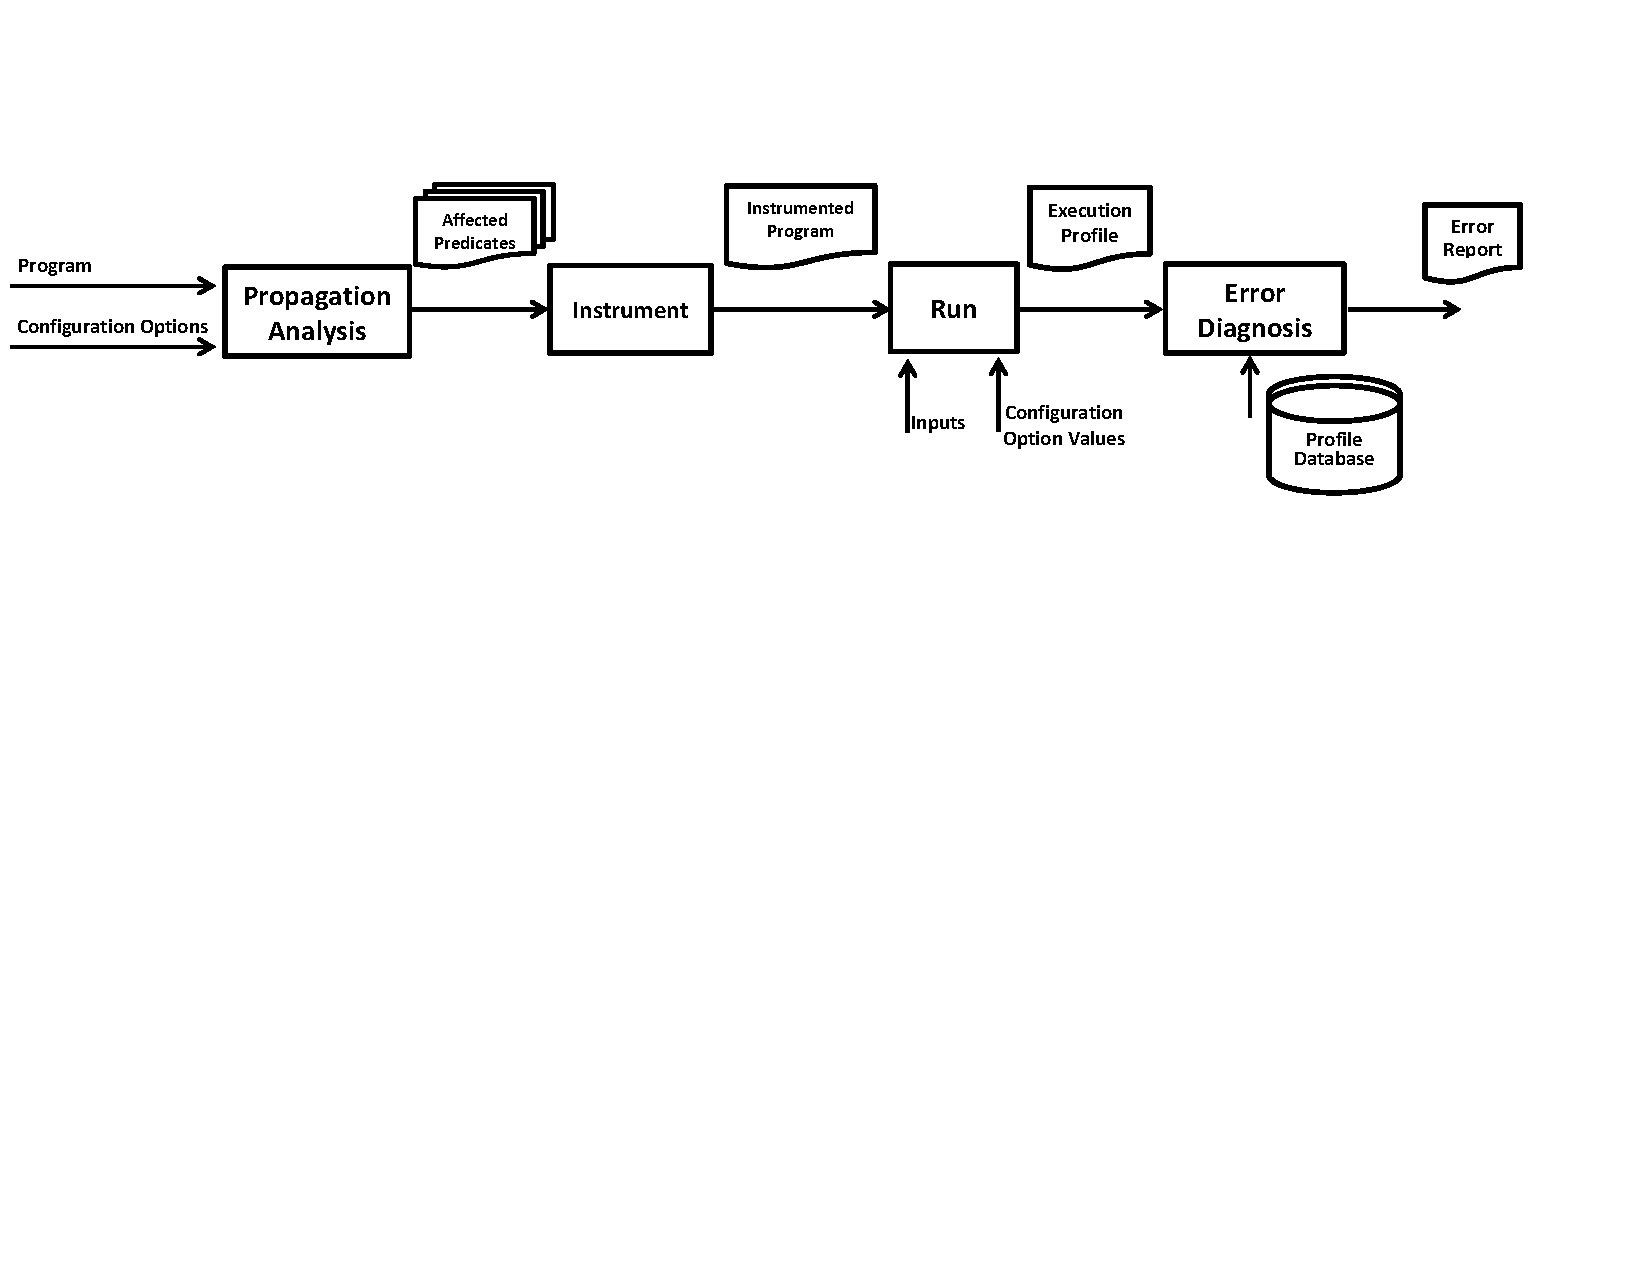
\includegraphics[scale=0.600]{architecture}
  \vspace*{-2.0ex}\caption {{\label{fig:workflow} The workflow of our configuration error diagnosis technique.
``Propagation Analysis'' is described in Section~\ref{sec:prop}.
The ``Instrument'' and ``Run'' components correspond to the Configuration Behavior Profiling step in Section~\ref{sec:profiling}.
``Deviation Analysis'' is described in Section~\ref{sec:analysis}.
}}
%\todo{The paper sometimes uses the terminology ``execution profile'' and
%  sometimes ``trace''.  Please be consistent.  I like ``execution profile''
%  better, because there is no temporal information about ordering in it.}
%\todo{The use of ``inputs'', in this figure and elsewhere, suggests that
%  the user runs multiple executions.  In fact, it is one execution, right?
%  I would change the arrow label ``inputs'' to ``input'' and
%  ``configurations'' to ``configuration''.  I would also label them as
%  ``bad runs''.  Then, I would change the database symbol's label from
%  ``Profile Database'' to ``Profile Database (good runs)''.}
\end{figure*}

\label{dummy-for-etags-workflow}


%\vspace{1mm}
%\noindent \textbf{\textit{Evaluations.}} 

\subsection{Evaluation}

We evaluated \ourtool on \errors real configuration errors
(\crash crashing errors and \noncrash non-crashing errors)
from \subjectnum projects.
On average, \ourtool's 5th report was the root cause; in
\topnum out of \errors cases, the root cause was \ourtool's
top 3 reports; and in over half of all
cases, the root cause was \ourtool's first report.
% This permits \ourtool user to focus on a few specific configuration
% options when deciding how to fix the problem. 
Assuming the database of correct execution profiles already exists,
\ourtool takes less than \avgtime minutes on average to diagnose
one error.  \ourtool's accuracy and speed make it an attractive alternative
to manual debugging.

%\todo{Defer most or all of the below details, especially ones related to
%  internal implementation choices.  This is too many low-level details at
%  this point in the paper.}

We compared \ourtool to an existing technique, called ConfAnalyzer~\cite{Rabkin:2011:PPC},
which uses dynamic information flow analysis to reason about the root cause of a
configuration error. \ourtool produced better results for 8 errors,
equivalent results for 3 errors, and worse results for 3 errors.

%As a result, \ourtool produced accurate diagnosis information for the \noncrash
%non-crashing errors that ConfAnalyzer failed to diagnose,
%and produced better or the same results
%for 6 out of the \crash crashing errors. 

We also compared \ourtool to two techniques leveraging
existing fault localization techniques~\cite{Jones:2002, McCamant:2003}
to diagnose configuration errors. 
\ourtool significantly outperformed both of them.

%\todo{Should I add this sentence: suggesting the necessity of
%designing new configuration error diagnosis techniques. Seems a bit
%verbose}
%, suggesting
%the necessity of designing new configuration error diagnosis techniques.% such as \ourtool.

%three variants and one existing
%technique, .
%The three variants is based on \ourtool, but use different
%abstractions rather than
%the affected predicates as computed by thin slicing in
%error diagnosis. ConfAnalyzer, one of the most precise
%configuration error diagnosis technique, uses dynamic
%Our experimental results show that \ourtool significantly
%outperformed three variants.
%Compared to ConfAnalyzer,



Finally, we evaluated two internal design choices of \ourtool.
First, we show that using thin slicing~\cite{Sridharan:2007} to compute the affected
predicates yielded more accurate diagnosis than using full slicing~\cite{Horwitz:1988}.
Second, we %investigated the effects of varying the comparison execution profiles from \ourtool's database, and
show that varying the execution
profile selection strategy can result in substantially different
results. %, depending on the application being analyzed;
The similarity-based selection strategy used in \ourtool outperformed
the other two strategies.


%\ourtool outputs an ordered list of probable root causes.
%Each entry in the list is a user-settle configuration option;
%our results show that \ourtool typically outputs
%the actual responsible configuration option as the top 3 in the list.

%By finding the
%needle in the haystack, \ourtool can be an attractive ...

%While xxx analysis takes a few minutes for a complex application,
%automated error diagnosis is still considerably faster and
%less labor-intensive than manual debugging or searching
%through other resources.

%$\blacksquare$ our technique is lightweighted.

%\vspace{1mm}
%\noindent \textbf{\textit{Contributions.}}


\subsection{Contributions}
This paper makes the following contributions:

\begin{itemize}
%\item \textbf{Problem.} To the best of our knowledge, we are the first to address
%the invalid thread access error detection problem for multithreaded GUI applications.

\item \textbf{Technique.} We present a technique to diagnose
software configuration errors. Our technique uses static analysis,
dynamic profiling, and statistical analysis to link the
undesired behavior to specific configuration options (Section~\ref{sec:technique}).


\item \textbf{Implementation.} We implemented our technique 
in a tool, called \ourtool, for Java software (Section~\ref{sec:implementation}). It is available at
\url{http://config-errors.googlecode.com}. 


\item \textbf{Evaluation.} We applied \ourtool to diagnose
\errors configuration errors in \subjectnum
configurable Java software projects. The results
show the usefulness of the proposed technique (Section~\ref{sec:evaluation}).

\end{itemize}




% LocalWords:  misconfigurations NanoXML maxsize newSequence GenInputsAbstract
% LocalWords:  randoop ForwardGenerator pre readFromCommandLine eSeq currSeq
% LocalWords:  ExecutableSequence createNewUniqueSequence AbstractGenerator
% LocalWords:  executionVisitor processSequence componentManager ConfAnalyzer
% LocalWords:  addGeneratedSequence
